\section{Làm việc với BE-PUM}

Trong BE-PUM có xây dựng một hệ thống mô tả môi trường làm việc tương tự như trên một hệ thống máy tính khởi chạy ngoài thực tế; chúng bao gồm các thành phần chính mà đề tài sẽ ảnh hưởng đến như sau:

\begin{itemize}
\item 	\textbf{Chồng (stack)} là một đơn vị dùng để lưu trữ giá trị theo nguyên tắc xếp chồng lên nhau, hoạt động theo nguyên lý vào sau ra trước (Last In First Out (LIFO)). Nó được dùng với nhiều mục đích khác nhau, ví dụ như để ghi nhận địa chỉ cần trở về khi thực hiện gọi một chương trình con, hay để ghi nhận các giá trị của các tham số truyền vào khi gọi một hàm Windows API.\\

\item 	\textbf{Bộ nhớ (memory)} dùng để lưu trữ toàn bộ giá trị của các vùng nhớ mà chương trình đang làm việc. Windows API cũng có khả năng tương tác với phần này; do vậy, đòi hỏi khi xây dựng xử lý API cần đảm bảo kết quả chính xác cho thành phần này.\\

\item 	\textbf{Thanh ghi (register)} là một vùng nhớ có dung lượng nhỏ nhưng lại có khả năng truy xuất rất nhanh, chúng được dùng để làm vùng nhớ tạm, trung gian cho các câu lệnh chạy trong hệ thống. Mỗi khi gọi một hàm bất kỳ, nếu như kiểu trả về khác void thì giá trị trả về sẽ được lưu trữ vào thanh ghi EAX.\\
\end{itemize}


\section{Các câu lệnh hợp ngữ}

	\subsection{Assembly}
	
		\subsubsection{Bộ nhớ assembly}	
		 Biến và hằng trong assembly có tính chất và mục đích sử dụng khác nhau. Thông qua các câu lệnh liên kết chặn chẽ với bộ nhớ là các thanh ghi bộ nhớ, trạng thai, các cờ được đánh dấu mà thông qua đó để thực thi chương trình.\\

		Các thanh ghi bộ nhớ:		
		\begin{center}
			\begin{figure}[htp]
				\begin{center}
					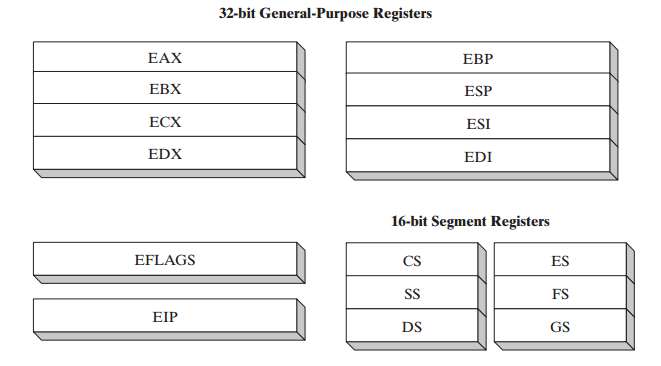
\includegraphics[scale=0.5]{ThanhGhi.png}
				\end{center}
				\caption{Thanh ghi (trính dẫn hình ảnh trong sách Assembly Language)}
				\label{fig:Flow}
			\end{figure}
		\end{center}
		
		Trong đó các thanh ghi General-Purpose gồm những thanh ghi có số bit nhỏ hơn:	
		\begin{center}
			\begin{figure}[htp]
				\begin{center}
					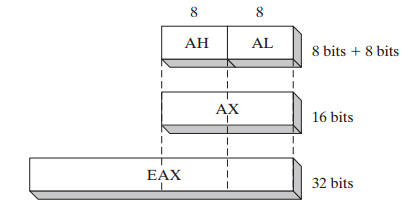
\includegraphics[scale=0.5]{ThanhGhi32bit.png}
				\end{center}
				\caption{Thanh ghi (trính dẫn hình ảnh trong sách Assembly Language)}
				\label{fig:Flow}
			\end{figure}
		\end{center}
		
		Ví dụ: thanh ghi EAX(32 bit địa chỉ) có thể được chia ra gồm thanh ghi AX(16 bit địa chỉ). Thanh ghi AX tiếp tục chia địa chỉ thành AH(8 bit) và AL(8 bit). Việc chia địa chỉ như thế giúp tối ưu bộ nhớ khi sử dụng.\\
		\begin{longtable}{ | m{3cm} | m{3cm} | m{3cm}  | m{3cm}| }
			\hline
				32 Bit & 16 Bit & 8Bit & 8 Bit\\
			\hline
			\hline
				EAX & AX	& AH	 & AL\\
			\hline			
				EBX & BX	& BH	 & BL\\
			\hline		
				ECX & CX	& CH	 & CL\\		
			\hline
				EDX & DX	& DH	 & DL\\
			\hline
			\caption{Bảng chia bộ nhớ 32-bit, 16-bit, 8-bit}
			\label{table:tbthanhghi}
		\end{longtable}
		
			Đối với một số thanh ghi có 32-bit địa chỉ có thể chia ra 16-bit địa chỉ, không thể chia nhỏ hơn. Bảng chi bộ nhơ thanh ghi có thể chia ra 16-bit địa chỉ.\\
			\begin{longtable}{ | m{3cm} | m{3cm} | }
			\hline
				32 Bit & 16 Bit\\
			\hline
			\hline
				ESI & SI\\
			\hline			
				EDI & DI\\
			\hline		
				EBP & BP\\		
			\hline
				ESX & SP\\
			\hline
			\caption{Bảng chia bộ nhớ 32-bit,16-bit}
			\label{table:tbthanhghi}
		\end{longtable}
		
	Mỗi thanh ghi có một chức năng khác nhau: 
\begin{itemize}
	\renewcommand{\labelitemi}{\textbullet}
	\item	EAX: thường được sử dụng trong các phép tính số học: cộng, trừ, nhân, chia, các phép toán logic, chuyển dữ liệu.
	\item EBX: được sử dụng như thanh ghi địa chỉ .
\item	ECX: được sử dụng trong các phép lặp, chuyển bit địa chỉ, xoay bit địa chỉ.
\item	EDX: thường được dùng để lưu dữ liệu, kết hợp vơi thanh ghi EAX thực hiện các phép toán nhân, cộng.
\item	ESP: luôn trỏ thới địa chỉ đỉnh stack hiện thời.
\item	EBP: thanh ghi dùng để truy cập giá trị, nhập dữ liệu stack. Khác với thanh ghi ESP, thanh ghi EBP còn được sử dụng để truy cập trong các đoạn chương trình khác nhau.
\item	EIP: thanh ghi con trỏ chỉ dẫn, giá trị của thanh ghi không thể thay đổi một các trực tiếp, chỉ thay đổi khi trỏ tới câu lệnh tiếp theo. Thanh ghi EIP lưu giá trị trỏ tơi của câu lệnh tiếp theo sẽ được gọi. 
\item	ESI, EDI: thanh ghi chỉ số nguồn và chỉ số đích thường được dùng trong các thao tác, xử lý mảng và chuỗi.
\end{itemize}	
	
	Thanh ghi EFLAGS bao gồm các chuỗi nhị phân được điều khiển bởi CPU hoặc phản ánh một số phép toán của CPU. Trạng thái của CPU. Bao gồm 8 cờ hiệu với mỗi loại cờ có chức năng khác nhau:
\begin{itemize}
	\renewcommand{\labelitemi}{\textbullet}		
		\item CF(Carry Flag cờ nhớ): cờ được bật khi phép tính có nhớ bit.
		\item ZF(Zero Flag cờ 0): cờ được bật khi phép tính vừa thực hiện là 0.
\item SF(Sign Flag cờ dấu): cờ này được bật khi kết quả thực phép tính có bit dấu.
\item	OF(Overflow Flag cờ tràn): cờ được bật khi kết quả thực hiện phép tính bị tràn số học.
\item	PF(Parity Flag cờ chẵn lẽ): cờ được bật khi kết quả của phép tính có chẵn bit 1.
\item	AF(Auxilary Flag cờ nhớ phụ): cờ được bật khi phép tính được thực hiện có sử dụng bit nhớ phụ.
\item IF(Interrupt Flag cờ ngắt): cờ được bật khi có thông báo cho phép ngắt xảy ra.
\item DF(Direction Flag cờ hướng): cờ được bật và sử dụng khi thao tác với mảng và chuỗi, sử dụng để giảm chỉ số tự động thi thao tác.
\end{itemize}	

		\subsubsection{Câu lệnh assembly}
		Một câu lệnh assembly có cú pháp đầy đủ như sau: 
		 \begin{center}		 
			\fontshape{it}  
			\selectfont
		 	$[ $ Nhãn lệnh: $]$  	$<$ Tên lệnh $<$ 	$[$ Các toán hạng $]$	$[$ ;lời chú thích $]$ \\
		 \end{center}			
		Trong đó:
		
		\begin{itemize}
		\renewcommand{\labelitemi}{\textbullet}		
		\item $[$ Nhãn lệnh: $]$  là một chuỗi ký tự kết thúc bằng dâu “:”, được thanh thế cho địa chỉ câu lệnh, được sử dụng trong câu lệnh If, else hoặc cần gọi thay bằng địa chỉ câu lệnh. Trong một chương trình không thể có hai nhãn lệnh trùng tên, tên nhãn lệnh không được trùng với tên thủ tục.
		\item $<$Tên lệnh $>$là một trong số những lệnh gợi nhớ của mã assembly, không phân biệt chữ hoa, chữ thường. Mỗi dòng lệnh chỉ đảm nhận một câu lệnh, mỗi câu lệnh phải được đặt trên một dòng.
		\item $[$Các toán hạng$]$ là các đối tượng mà câu lệnh sẽ tác động vào. Tùy theo từng câu lênh mà có 0 toán hạng, 1 toán hạng, 2 toán hạng, 3 toán hạng. Toán hạng đầu tiên gọi là toán hạng đích, toán hạng thứ 2 gọi là toán hạng nguồn. Với câu lệnh có 3 toán hạng thì chỉ có 1 toán hạng đích trong câu lệnh đó. 
		\item $[$; lời giải thích$]$ khi biên dịch thì lời giải thích không được biên dịch sang mã máy, chỉ có tác dụng với người đọc chương trình. Giúp người đọc dễ hiểu các câu lệnh.
		\end{itemize}

	Ví dụ 1: xét câu lệnh sau đây: 
	 \begin{center}		 
		VD1: mov ax, bx	;lưu giá trị thanh ghi ax từ thanh ghi bx
	\end{center}
	Trong đó:
	\begin{itemize}
		\renewcommand{\labelitemi}{\textbullet}			
	  \item	VD1 : là chuỗi ký tự nhãn lệnh.
	\item	mov: tên lệnh với chức năng lưu giá trị đích(ax) từ giá trị nguồn (bx).
	\item	ax, bx: các toán hạng, trong trường hợp này là các thanh ghi bộ nhớ 16 bit.
	\item $;$ lưu giá trị thanh ghi ax từ thanh ghi bx : lời giải thích, chú thích thêm.
	\end{itemize}
	
	Xem các câu lệnh sau đây:
	\begin{itemize}
	\renewcommand{\labelitemi}{\textbullet}		
	\item  NOT	: đây là câu lệnh không có toán hạng.
	\item	Mov ax, bh: câu lệnh này có 2 toán hạng ax (toán hạng đích) thanh ghi 16 bit, bh (toán hạng nguồn) thanh ghi 8 bit.
	\item	Add ah, sqt: câu lệnh này có 2 toán hạng ah (toán hạng đích) thanh ghi 8 bit, sqt (toán hạng nguồn) một biến được gán trước có kiểu dữ liệu là byte.
	\item	Mov ax, [SI]: câu lệnh này có 2 toán hạng ax (toán hạng đích) thanh ghi 16 bit, [SI] (toán hạng nguồn) là một ô nhớ.
	\item	Imul ax, bx, 10: câu lệnh này có 3 toán hạng ax (toán hạng đích) thanh ghi 16 bit, bx (toán hạng nguồn) thanh ghi 16 bit, và một hằng số (10).
	\end{itemize}

	Câu lệnh Imul có tới 3 toán hạng, toán hạng đích (ax) sẽ được lưu kết quả của phép nhân từ toán hạng nguồn (bx) nhân với hằng số (10: tức toán hạng thứ 3).\\
	Bảng ký hiệu toán hạng:
	\begin{longtable}{ | m{3cm} | m{12cm} | }
			\hline
				Toán hạng & 16 Mô tả\\
			\hline
			\hline
				reg8 & Thanh ghi có 8 bit địa chỉ: AH, AL, BH, BL, CH, CL, DH, DL \\
			\hline			
				reg16& Thanh ghi có 16 bit địa chỉ: AX, BX, CX, DX, SI, DI, SP, BP\\
			\hline		
				reg32& Thanh ghi có 32 bit địa chỉ: EAX, EBX, ECX, EDX, ESI, EDI, ESP, EB\\
			\hline	
				reg&	Bất kỳ thanh ghi nào\\
			\hline	
				sreg & Thanh ghi segment có 16 bit địa chỉ: CS, DS, SS, ES, FS, GS\\
			\hline	
				imm	&8- , 16-, hoặc 32- bit giá trị được truyền vào\\
			\hline	
				imm8	& Giá trị hằng số truyền vào kiểu byte 8-bit\\
			\hline	
				imm16	& Giá trị hằng số truyền vào kiểu word 16-bit\\
			\hline	
				imm32&	Giá trị hằng số truyền vào kiểu doubleword 32-bit\\
			\hline	
				reg/mem8& Toán hạng 8 bit, có thể là thanh ghi có 8-bit địa chỉ hoặc bộ nhớ byte\\
			\hline	
				reg/mem16&	Toán hạng 16 bit, có thể là thanh ghi có 16-bit địa chỉ hoặc bộ nhớ word\\
			\hline	
				reg/mem32	& Toán hạng 32 bit, có thể là thanh ghi có 32-bit địa chỉ hoặc bộ nhớ doubleword\\
			\hline	
				mem	& Bất kỳ bộ nhớ 8-, 16-, 32- bit\\
		\hline	
			\caption{Bảng ký hiệu toán hạng:}
			\label{table:tbkyhieu}
	\end{longtable}
	
		Phân tích câu lệnh mov: \\
		Cú pháp: 
		\begin{itemize}
			\renewcommand{\labelitemi}{\textbullet}	
			\item Mov [toán hạng đích], [toán hạng nguồn].
			\item	Mov reg/mem8, reg8
			\item Mov reg/mem16, reg16
			\item	Mov reg/mem32, reg32
			\item	Mov reg8, reg/mem8
			\item	Mov reg16, reg/mem16
			\item	Mov reg32, reg/mem32
			\item	Mov reg/mem16, sreg
			\item	Mov sreg, reg/mem16
			\item	Mov reg8, imm8
			\item	Mov reg16, imm16
			\item	Mov reg32, imm32
			\item	Mov reg/mem8, imm8
			\item	Mov reg/mem16, imm16
			\item	Mov reg/mem32, imm32	
		\end{itemize}
	
	Trong đó: 
	\begin{itemize}
		\renewcommand{\labelitemi}{\textbullet}	
			\item  $[$ Toán hạng đich$]$: có thể là thanh ghi (8 bit, 16 bit, 32 bit), ô nhớ (địa chỉ của ô nhớ) hay một biến nào đó.$[$Toán hạng đích$]$không thể là hằng số.
			\item $[$ Toán hạng nguồn $]$: có thể là hằng số, biến, thanh ghi, ô nhớ.
	\end{itemize}

	Xem ví dụ sau:
		\begin{itemize}
		\renewcommand{\labelitemi}{\textbullet}	
		\item	Mov ax, bx 		; đặt giá trị của thanh ghi bx vào ax.
		\item Mov ax, 5		; đặt giá trị 5 vào thanh ghi ax.
		\item	Mov bx, 5*3 		; đặt giá trị 5*3 vào thanh ghi bx.
		\item Mov DI, ‘A’		; đặt mã ASCII của ‘A’ vào thanh ghi DI
		\item Mov ch, var		; đặt giá trị của biến var kiểu byte vào thanh ghi ch.
		\item	Mov bh, 300		; giá trị không hợp lệ vì bh có kiểu byte giới hạn 255 nên không thể gán giá trị 300 vào bh.
		\item	Mov ch, ax		; giá trị không hợp lệ vì giá trị thanh ghi ax (16 bit) không thể gán giá trị vào thanh ghi ch (16 bit).  
		\end{itemize}

		\subsubsection{Tập giá trị}
		Khác với các ngôn ngữ lập trình khác, kiểu giá trị của assembly có đôi chút khác biệt, được tính theo bit, tùy theo yêu cầu sử dụng của người lập trình. \\
		Các kiểu dữ liệu:
		\begin{longtable}{ | m{3cm} | m{8cm} | }
			\hline
				Kiểu & Cách sử dụng\\
			\hline
			\hline
				BYTE & 	kiểu số nguyên 8-bit không dấu.\\
			\hline
				SBYTE	& kiểu số nguyên 8-bit có dấu.\\
			\hline
				WORD& 	kiểu số nguyên 16-bit không dấu.\\
			\hline
				SWORD	& kiểu số nguyên 16-bit có dấu.\\
			\hline
				DWORD& 	kiểu số nguyên 32-bit không dấu.\\
			\hline
				SDWORD& 	kiểu số nguyên 32-bit có dấu.\\
			\hline
				FWORD	& kiểu số nguyên 48-bit.\\
			\hline
				QWORD& 	kiểu số nguyên 64-bit\\
			\hline
				TBYTE& 	kiểu số nguyên 80-bit (10-byte).\\
			\hline
				REAL4& 	kiểu số thực 32-bit (4-byte) chuẩn IEEE.\\
			\hline
				REAL8& 	kiểu số thực 64-bit (8-byte) chuẩn IEEE.\\
			\hline
				REAL10& 	kiểu số thực 80-bit (10-byte) chuẩn IEEE.\\			
			\hline
					\caption{Bảng kiểu dữ liệu:}
					\label{table:tbkieudulieu}
		\end{longtable}
		
		Ngoài ra còn có một số ký hiệu kiểu số tự nhiên.
		\begin{longtable}{ | m{3cm} | m{6cm} | }
			\hline
				Kiểu & Cách sử dụng\\
			\hline
			\hline
				DB &	kiểu số nguyên 8-bit.\\
			\hline
				DW &	kiểu số nguyên 16-bit.\\
			\hline			
				DD &	kiểu số nguyên hoặc số thực 32-bit.\\
			\hline
				DQ	 &kiểu số nguyên hoặc số thực 64-bit.\\
			\hline
				DT	 &định nghĩa kiểu số nguyên 80-bit (10 byte).\\
			\hline
					\caption{Bảng ký hiệu kiểu số tự nhiên:}
					\label{table:tbkieudulieutn}
		\end{longtable}
		
		Trên cở sở các đơn vị dữ liệu được lưu trên kiến trúc X86, một byte tưng ứng với 8-bit, tưng tự word tưng ứng với 16-bit (2 byte), doubleword tưng ứng với 32-bit (4 byte), quadword tưng ứng với 64-bit (8 byte). Từ đó ta tính toán được phạm vi giới hạn số học của các kiểu số nguyên không dấu và có dấu: 
			\begin{longtable}{ | m{5cm} | m{6cm} | m{3cm} |}
			\hline
				Kiểu lưu trữ &	Phạm vi (từ thấp đến cao)&	Dung lượng\\
			\hline
			\hline
				Byte không dấu &	0 đến 255&	1 byte\\
			\hline
				Word không dấu	&0 đến 65,535&	2 bytes\\
			\hline
				Double word không dấu	 &0 đến 4,294,967,295&	4 bytes\\
			\hline
				Quadword không dấu	&0 đến 18,446,744,073,709,551,615&	8 bytes\\
			\hline
				\caption{Bảng phạm vi kiểu dữ liệu số không dấu}				
			\end{longtable}
		
			\begin{longtable}{ | m{5cm} | m{7cm} |}
			\hline
				Kiểu lưu trữ	& Phạm vi (từ thấp đến cao)\\
			\hline
			\hline
				Byte có dấu	& -128 đến +127\\
			\hline
				Word có dấu &	-32,768 đến +32,767\\
			\hline	
				Double word có dấu &	-2,147,483,648 đến +2,147,483,647\\
			\hline	
				Quadword có dấu	 & -9,223,372,036,854,775,808 đến +9,223,372,036,854,775,807 \\
			\hline
			\caption{Bảng phạm vi kiểu dữ liệu số có dấu}				
			\end{longtable}		
		
		\subsubsection{Kiếu giá trị}
		\subsubsection*{Hằng số}
		Kiểu hằng số nguyên được dùng trong hợp ngữ assembly là một chuỗi số đứng trước nó là dấu của số nguyên đó, tiếp theo là chuỗi số và cuối cùng là cơ số để xác định chuỗi số đó. Cú pháp của chuỗi số:		
		\begin{center}
			\fontshape{it}  
			\selectfont
		 	$[{+|-}]$ chuỗi số$ [$cơ số$]$
		\end{center}
	
	Cơ số là một trong những dạng cơ số dưới đây (không phân biệt chứ hoa hay chữ thường):
		\begin{itemize}
		\renewcommand{\labelitemi}{\textbullet}	
			\item	h	: Hexadecimal hệ cơ số 16
			\item	q/o	: Octal hệ cơ số 8
			\item	d	: Decimal hệ cơ số 10
			\item	b	: Binary hệ cơ số 2
		\end{itemize}			
	Nếu không có ký hiệu cơ số thì mặc định số đó là hệ cơ số 10. Dưới đây là một số ví dụ:
	\begin{itemize}
	\item	26		: 26 hệ cơ số 10
	\item	26d		: 26 hệ cơ số 10
	\item	11010011b	: 11010011 hệ cơ số 2
	\item	42q		: 42 hệ cơ số 8
	\item	42o		: 42 hệ cơ số 8
	\item	1Ah		: 1A hệ cơ số 16
	\end{itemize}	
	
	\subsubsection*{Biểu thức số nguyên}
	Biểu thức số nguyên là các biểu thức toán học mà các toán hạng thuộc kiểu số nguyên. Các biểu thức toán học được xếp theo thứ tự ưu tiên, việc xếp thứ tự này khá quan trọng vì nó ảnh hưởng đến kết quả của một biểu thức. Dưới đây là bảng biểu thức toán học được sắp thứ tự ưu tiên cao nhất là 1 và thấp nhất là 4:	\\
	\begin{longtable}{ | m{3cm} | m{5cm} |m{5cm} |}
			\hline
				Toán tử &	Tên &	Thứ tự ưu tiên\\
			\hline
			\hline
			$()$	 &	Dấu ngoặc&		1\\
			\hline
			$+, -$ &		Dấu dương, âm&		2\\
			\hline
			$*, /$	&	Nhân, chia&		3\\
			\hline
			MOD	&	Chia lấy dư&		3\\
			\hline
			$+,-$	&	Cộng, trừ	&	4\\
			\hline
			\caption{Thứ tự ưu tiên biểu thức toán}
	\end{longtable}
	Xem các ví dụ dưới đây để hiểu rõ hơn:
	\begin{itemize}
	\item  4 $+$ 5 $*$ 3 		: Thực hiện phép nhân trước khi thực hiện phép cộng
	\item	 12 – 2 MOD 3	: Thực hiện phép chia lấy dư trước khi thực hiện phép trừ
	\item	 $-$7 $+$ 2			: Lấy dấu của số 7 trước khi thực hiện phép cộng với 2
	\item	$($5 $+$ 3$) *$ 7		: Thực hiện biểu thức trong ngoặc trước khi thực hiện phép nhân. 
	\end{itemize}
	
	\subsubsection*{Kiểu ký tự và chuỗi}
	Kiểu ký tự và chuỗi ký tự trong hợp ngữ assembly dựa trên bảng mã ASCII để xây dựng. Biến có kiểu ký tự được lưu dưới dạng mã nhị phân của bảng mã ASCII. 
	Cách khai báo biến có kiểu ký tự:
	\begin{itemize}
		\item	‘A’ 
		\item	“b” 
	\end{itemize}
	Một chuỗi ký tự được đặt trong dấu nháy đơn (‘’)  hoặc nháy kép (“”):
	\begin{itemize}		
		 \item  ‘ABCDEF’
		\item	“AAAA”
		\item	“Hom nay la thu hai”
		\item	‘123456’ 
	\end{itemize}	
		
		\subsubsection{Cấu trúc một chương trình assembly}
			Hiện này, hầu hết các hệ điều hành hiện nay, đặc biệt là hệ điều hành Microsoft đều hỗ trợ hai dạng cấu trúc tập tin thực thi là COM và EXE. Nhưng trong BE-PUM tập trung phân tích cấu trúc tập tin EXE. Cấu trúc tập tin EXE và COM có sự khác biệt rất lớn. Cấu trúc tập tin EXE được chia thành ba đoạn: Mã lệnh (Code), dữ liệu (Data), ngăn xếp (Stack). Trong khi đó cấu trúc tập tin COM chỉ có một đoạn mã lệnh được gom từ ba đoạn trong cấu trúc tập tin EXE. \\

Ngoài ra, cấu trúc tập tin EXE có thể bố trí hơn ba đoạn bộ nhớ. Do đó, khi thiết kế chương trình, hay gặp phải chương trình được bố trí hơn ba đoạn thì cần phải quan tâm đến các modun của chương trình, sự liên kết giữa các đoạn với nhau. \\

Cấu trúc chương trình được giới thiệu, phân tích dưới đây là cấu trúc tập tin thực thi EXE, nêu lên những khái niệm cơ bản của một chương trình assembly. \\
	\begin{normalsize}
			\setlength{\parindent}{1cm}		
			\renewcommand{\rmdefault}{cmss}
			\textit {$.$ Model	$<$ chế độ bộ nhớ $>$	}		\\	
			\indent  \textit{.Stack 100h } \\			
			\indent \textit{<khai báo dữ liệu>} \\			
			\indent \textit{.Code}\\
			\indent \textit{<Thủ tục chính > PROC}\\ \\
			\indent \textit{<các câu lệnh của chương trình>}\\ \\
			\indent \textit{< Thủ tục chính> } \\
			\indent \textit{Endp}\\
			\indent \textit{<Các thủ tục khác được khai>}\\
			\indent \textit{END}\\
	\end{normalsize}
	
	Trong cấu trúc được đưa ra, các từ \textit {.Model, .Stack, .Data, .Code, PROC, Endp, END} là các từ để hướng dẫn thực thi một chương trình assembly. \\

Nhìn vào cấu trúc chương trình, ta thấy rõ một chương trình assembly được phân tích ra gồm 3 đoạn chính: đoạn \textit{Code}, chứa toàn bộ mã lệnh, nơi thực thi của chương trình, đoạn \textit{Data} nơi chứa các biến dữ liệu được khai báo của chương trình, đoạn Stack nơi chứa stack của chương trinh khi chương trình được nạp vào bộ nhớ để thực thi.\\

Hướng dẫn \textit{.Model} được đạt ngay trên đầu của cấu trúc chương trình nhằm mục đích khai báo chế độ nhớ mà chương trình sử dụng để thực thi.\\

Hướng dẫn \textit{.Stack} đặt ở đầu chương trình mục đích để khai báo kích thước stack được sử dụng để thực thi chương trình. Kích thước stack thường được khai báo là 100h (256) byte.\\

Ví dụ chương trình được viết theo cấu trúc EXE:\\
	\begin{normalsize}
			\setlength{\parindent}{1cm}		
			\renewcommand{\rmdefault}{cmss}
				\textit {.model small}
     			\textit { include \textbackslash masm32 \textbackslash include \textbackslash windows.inc}  \\  
				\textit { include \textbackslash masm32 \textbackslash include \textbackslash windows.inc} \\
				\textit { include \textbackslash masm32 \textbackslash include \textbackslash windows.inc} \\
				\textit { include \textbackslash masm32 \textbackslash include \textbackslash windows.inc} \\ \\
				\textit { include \textbackslash masm32 \textbackslash include \textbackslash windows.inc} \\ 
				\textit { include \textbackslash masm32 \textbackslash include \textbackslash windows.inc} \\
				\textit { include \textbackslash masm32 \textbackslash include \textbackslash windows.inc} \\
				\textit { include \textbackslash masm32 \textbackslash include \textbackslash windows.inc} \\
				\textit {stack 100h}\\
				\textit {.data}\\
				\textit {var1 WORD  200}\\
				\textit {.code}\\
				\textit {start: }\\
    			\textit {main proc}\\
        		\textit {mov ax, 775}\\
       			 \textit {aad   }\\
        		\textit {	mov eax, 100 }\\
       			\textit { aad}\\
        		\textit {	mov bl, 5}\\
        		\textit {	div bl   }\\
				\textit {mov eax, 10}\\
   				\textit {bsf eax, var1}		\\
		  		\textit {ret}\\
     			\textit {main endp}\\
				\textit {end start}\\
	\end{normalsize}
	
		Ở phần đầu chương trình có khai báo các đường dẫn thư viện hỗ trợ chương trình bằng cú pháp:
		\begin{center}
			\textit { include <đường dẫn>} \\
		\end{center}
					
	Có thể thấy đoạn chương trình trên sử dụng chế độ bộ nhớ Small. Khai báo kích thước Stack là 100h byte. Trong phần khai báo dữ liệu Data chỉ khai báo một biến duy nhất là var1 có kiểu dữ liệu là word, giá trị của biến là 200. Trong phần Code, tên thủ tục là main, tên thủ tục có thể được đặt tùy ý.\\


	\subsection{Floating-Point Unit (FPU)}
	Kiên trúc Floating-Point Unit (FPU) của Intel cung cấp hiệu quả cao trong khả năng xử lý floating-point. Kiến trúc FPU hỗ trọ xử lý các số nguyên, số thực và Biniary Coded Decimal (BCD)-số nguyên kiểu dữ liệu, và các floating-point được sử lý bằng thuật toán được định nghĩa theo tiêu chuẩn IEEE 754 và 854. Các câu lệnh FPU được thực hiện từ bộ vi sử lý của các dòng lệnh bình thường và được cải thiện đáng kể hiệu quả của các bộ vi xử lý Intel trong xử lý các phép tính có độ chính xác cao, các hoạt động xử lý dấu chấm động.\\
		\subsubsection{Số thực và định dạng Floating-point}	
		Phần này sẽ mô tả cách các số thực được biểu diễn ở dạng dấu chấm động của FPU trong kiến trúc Intel. Đồng thời giới thiệu các thuật ngữ như số normalized, số denormalized, số mũ, số không, và NaN (not a number). 
		
		\subsubsection*{Hệ thống số thực}
		Như thể hiện trong hình 3, hệ thống số thực bao gồm sự liên tục của các số thực từ trừ vô cực (-$\mathbb{\infty}$)  đến cộng vô cực (+$\mathbb{\infty}$) .\\
		\begin{center}
			\begin{figure}[htp]
				\begin{center}
					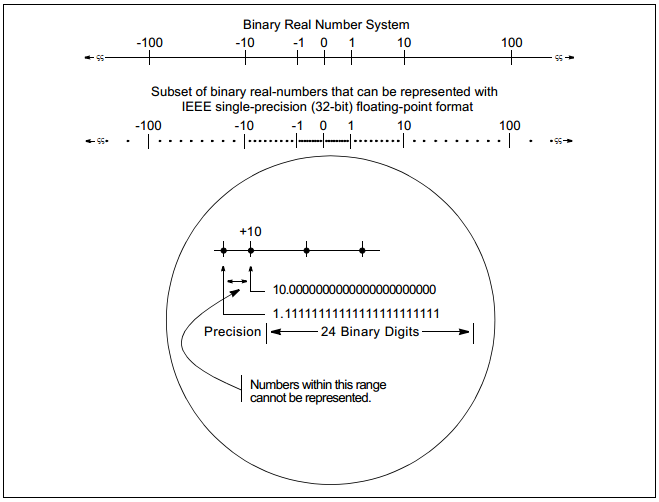
\includegraphics[scale=0.8]{MaNhiPhan.png}
				\end{center}
				\caption{Hệ thống mã nhị phân biểu diễn số thực}				
			\end{figure}
		\end{center}		
		
		Bởi vì kích thước và số lượng thanh ghi của bất kỳ máy tính nào có thể có hạn chế, chỉ có một đoạn mã nhị phân của số thực có thể được sử dụng trong tính toán số thực. Hình 3, phần số thực mà FPU hỗ trợ biểu diễn một giá trị xấp xỉ của một số thực. Phạm vi và độ chính xác của các phần mã nhị phân của số thực được biểu diễn theo định dạng FPU sử dụng để hiện thi cho số thực được sử dụng.
		
		\subsubsection*{Định dạng Floating-point}
		Để tăng tốc độ và hiệu quả của các phép tính số thực, các FPU hiện thị đại diện cho một số thực mà được biểu diễn theo định dạng floating-point. Trong định dạng này, một số thực có ba phần: bit dấu, định trị và số mũ. Định dạng này phù hợp với chuẩn IEEE.\\
		\begin{center}
			\begin{figure}[htp]
				\begin{center}
					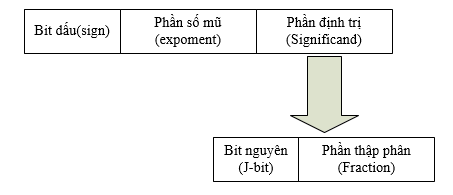
\includegraphics[scale=0.8]{DinhDangMNP.png}
				\end{center}
				\caption{Định dạng mã nhị phân của Floating-point}				
			\end{figure}
		\end{center}		
		
		Bit dấu là một giá trị nhị phân cho biết xem số đó là số âm (1) hay số dương (0). Phần định trị gồm hai phần: bit số nguyên (J-bit) và phần phân số. Phần bit số nguyên thường không được hiện thị, nhưng thay vào đó có giá trị mặc định. Phần số mũ là một số nguyên biểu diễn lũy thừa 2, điều này làm cho phần định trị được tăng lên.
		
		\subsubsection*{Số thông thường (normalized)}	
		Trong hầu hết mọi trường hợp, thanh ghi FPU hiển thị giá trị số thực định dạng thông thường. Ngoại trừ số 0 thì phần định trị luôn được tạo bởi một số thực và theo sau là phần phân số.
		\begin{itemize}
			\item[•	]1.fff…fff
		\end{itemize}
				
	\begin{longtable}{ | m{7cm} | m{7cm} | }
		\hline
				Ký hiệu & Giá trị\\
		\hline
		\hline
			Số thập phân	&178.125\\
		\hline	
			Số thập phân khoa học&	1.78124E102\\
		\hline	
			Số nhị phân khoa học	&1.0110010001E2111\\
		\hline	
			Số nhị phân khoa học (biểu diễn số mũ)	&1.0110010001E210000110\\
		\hline
			Đinh dạng số thực & 0(Bit dấu)  10000110(Phần mũ)	 011001000100000000000001(Phần định trị)\\
		\hline
	\end{longtable}		
		
		Đối với các giá trị thấp hơn 1 thì số 0 ở phia trước được loại bỏ (mỗi số 0 được loại bỏ, số mũ được tăng lên 1).\\

		Để hiện thị số lớn nhất của phần định trị theo định dạng thông thường thì phải cung cấp độ dài của phần định trị này. Để hiện thị số thực theo định dạng thông thường này thì phần định trị sẽ biểu diễn giá trị giữa 1 và 2, phần số mũ sẽ chỉ ra độ tăng của số thực đó.
		
		\subsubsection*{Số mũ (baised expoment)}
			Thanh ghi FPU biểu diễn số mũ theo định dạng cơ bản. Có nghĩa là một hằng số sẽ được thêm vào số mũ được biểu diễn vì vậy số mũ luôn là một số dương. Giá trị hằng số phụ thuộc vào số lượng bit được dùng để biểu diễn số thực trong định dạng dấu chấm phẩy động được sử dụng. Hằng số được chọn sao cho có thể thay đổi giá trị nhưng vẫn không bị tràn số.
			
			\subsubsection*{Số thực và mã hóa phi số thực}
			Có nhiều loại số thực và giá trị đặc biệt có thể được mã hóa theo định dạng dấu phẩy động của FPU:\\
			
			Những số đặc biệt và giá trị đặt biệt được chia thành các loại sau:
			\begin{itemize}
				\renewcommand{\labelitemi}{\textbullet}	
				\item Số 0.
				\item	Số hữu hạn không thông thường (denormalized).
				\item	Số hữu hạn thông thường (normalized).
				\item	Số vô cực
				\item	Không phải là một số (NaNs: Not a number )
				\item	Số không định nghĩa.
			\end{itemize}
			
			Hình ~\ref{fig:SothucNaN} sẽ chỉ rõ cách mã hóa số thực và phi số thực phù hợp với các biểu diễn số thực theo chuẩn IEEE. Ví dụ được sử dụng ở đây miêu tả chuẩn IEEE chính xác đơn (32-bit), các ký hiệu “S” chỉ bit dấu, “E” chỉ số mũ, “F” chỉ phần phân số. ( Giá trị của phần số mũ là một số nguyên). \\

		Các thanh ghi FPU có thể thực hiện các loại and/or trả về đúng giá trị, phụ thuộc vào phép toán được thực hiện. Các phần dưới đây sẽ mô tả các biểu diễn số thực và phi số thực.
		
		\subsubsection*{Số 0}
		Số 0 có thể được biểu diễn là +0 và  -0 phụ thuộc vào bit dấu. Việc mã hóa +0 và -0 tương đương nhau về mặt giá trị. Bít dấu của số 0 phụ thuộc vào phép toán được thực thi và cách thức làm tròn được sử dụng. Bit dấu số 0 có thể xác định tràn số dưới có đang xảy ra hay không, ngoài ra còn xác định bit dấu của giá trị vô cực. 
		
		\subsubsection*{Số normalized và denormalized}
		Trừ số 0, số thực được chia thành 2 dạng: normalized (bình thường) và denormalized (không bình thường). Số normalized bao gồm các giá trị khác 0, có thể mã hóa theo định dạng IEEE trong phạm vi từ số 0 đến vô cực. Trong hình 5, định dạng chính xác đơn với chỉ số mũ từ 0 đến 254 (phạm vi tham số -126 đến 126).
		\begin{center}
			\begin{figure}[htp]
				\begin{center}
					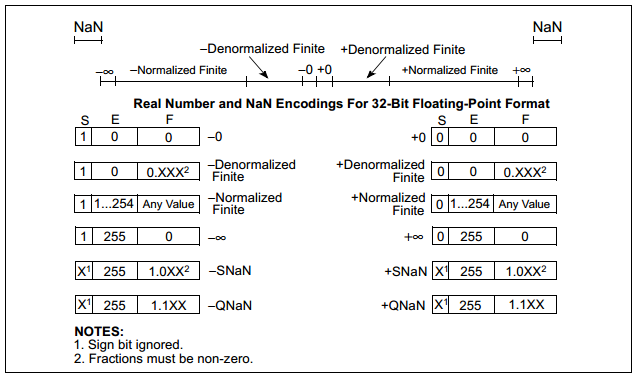
\includegraphics[scale=0.8]{SoThucNaN.png}
				\end{center}
				\caption{Số thực và NaN}				
				\label{fig:SothucNaN}
			\end{figure}
		\end{center}		

	Khi số thực càn gần về số 0, chiều dài bit dùng để biểu diễn số thực không đủ dài để biểu diễn. Bởi vì chỉ số mũ (trong ví dụ này là 32-bit) không đủ lớn để biểu diễn bit dịch phải để loại bỏ các bit 0 ở đầu (xem thêm phụ lục IEEE).\\

	Khi số mũ là số 0, những số nhỏ có thể được biểu diễn bằng những bit số nguyên (và những chuỗi bit ở đầu) của số 0. Số thực trong phạm vi này được gọi là denormalized (hay số rất nhỏ). Việc sử dụng các bit 0 ở đầu cho phép biểu diễn các số rất nhỏ nhưng những số rất nhỏ này là nguyên nhân mất đi sự chính xác (số bit trong phần định trị được giảm đi sẽ được tính toán dựa trên số bit 0 ở phần số mũ).\\

	Khi thực hiện các phép tính trên dấu chấm động, mỗi thanh ghi FPU thực hiện phép toán với số normalized và đưa ra kết quả là một số normalized. Số denormalized biểu diễn cho điều kiện tràn số dưới.\\
	
	Số denormalized được tính bằng kỹ thuật “gradual underflow”. Bảng () sẽ đưa ra một ví dụ của kỹ thuật “gradual underflow” trong xử lý tính toán số denormalized. Ở đây, sử dụng định dạng đơn nên số nhỏ nhất của số mũ là -126. Kết quả trong ví dụ này yêu cầu số mũ là -129. Nếu nhỏ hơn -129 là nằm ngoài phạm vi số mũ cho phép, kết quả của số denormalized bằng cách thêm các bit 0 ở đầu đến khi số mũ nhỏ nhất là -129.\\
		
		\begin{longtable}{ | m{4cm} | m{2cm} |  m{2cm} | m{4cm} | }
			\hline
				Toán hạng & Dấu & Số mũ* & Phần định trị\\
			\hline
			\hline
				Kết quả đúng & 0 & -129 & 1.01011100000..00\\
			\hline
				Số Denormalize & 0 & -128 & 0.10101110000..00\\
			\hline
				Số Denormalize & 0 & -127 & 0.01010111000..00\\
			\hline
				Số Denormalize & 0 & -126 & 0.00101011100..00\\
			\hline
				Kết quả Denormalize & 0 & -126 & 0.00101011100..00\\
			\hline
			\caption{Xử lý số denormalized}
		\end{longtable}
		
	
	Lưu ý: * Số mũ được biểu diễn trong phạm vi (-126 đến 126)\\

	Trong trường hợp tốt nhất, tất cả các bit của phần định trị được dịch phải bằng cách chèm thêm bit 0 ở đầu, tạo ra kết quả là số 0.\\

FPU xử lý với số demormal theo các cách sau đây: 
	\begin{itemize}
			\renewcommand{\labelitemi}{\textbullet}	
			\item	Không được phép tạo số denormalized.
			\item	Cung cấp xử lý ngoại lệ underflow để người lập trình có thể kiểm tra khi số denormalized được tạo ra.
			\item	Cung cấp các toán hạng xử lý số denormalized, cho phép chương trình kiểm tra khi mà các số denormalized được sử dụng như là một toán hạng. 
	\end{itemize}

	Khi một số denormalized ở định dạng chính xác đơn hoặc chính xác kép được sử dụng như một toán hạng, và xử lý ngoại lệ dernormal được đánh dấu, thanh ghi FPU sẽ tự động chuyển giá trị của số denormalized thành normalized bằng cách chuyển sang định dạng mở rộng.

		\subsubsection*{Số vô cực}
		Có 2 số vô cực là âm vô cực và dương vô cực được dùng để biểu diễn số thực âm nhỏ nhất và số thực dương lớn nhất vì vậy có thể biểu diễn dạng dấu chấm động. Số vô cực luôn được biểu diễn bằng bit 0 của phần định trị (phần phân số và bit số nguyên) và số mũ tối đa cho phép của mỗi định dạng (ví dụ: số mũ tối đa 255 đối với định dạng kép).\\

Bit dấu của số vô cực có thể dùng để so sánh. Số vô cực luôn được chỉ định rõ là âm vô cực luôn nhỏ hơn so với bất kỳ số thực cụ thể nào, dương vô cực luôn lớn hơn so với bất kỳ số thực cụ thể nào. Việc tính toán số vô cực luôn chính xác. Ngoại lệ được đánh dấu khi có phép toán xử dụng toán hạng là số vô cực, số vô cực được coi là toán hạng không hợp lệ. \\

Số denormalized biểu diễn cho điều kiện tràn số dưới, 2 số vô cực biểu diễn cho điều kiện tràn số trên. Kết quả số normlized của một phép toán có số mũ nằm trong phạm vi cho phép của số mũ phụ thuộc theo định dạng được sử dụng.
	
		\subsubsection*{NaNs (Not a number: không phải là một số)}
		NaN không phải là một, NaN là phần không nằm trên trục số thực trong hình 5. Việc mã hóa số NaN được chỉ ra trên trục số thực nằm ở cuối và đầu trục số. Khoảng trống này biểu diễn bất kỳ giá trị nào lớn với số mũ tối đa và phần phân số có bit khác không. (Bit dấu được bỏ qua đối với số NaN).\\

	Theo chuẩn IEEE có 2 định dạng cho NaN là: quiet NaNs(QNaNs) và signaling NaNs (SNaNs). Số QnaNs là NaN với phần phân số có hầu hết các bit là 1. Số SNaNs là NaN với phần phân số hầu hết các bit là 0. QNaNs cho phép tạo ra thông qua các phép toán mà không đánh dấu ngoại lệ nào. SNaNs thường thông báo một ngoại lệ không hợp lệ xảy ra khi thực hiện phép toán học. 
	
		\subsubsection*{Số không định nghĩa}
		Đối với mỗi loại dữ liệu của FPU, có một cách để mã hóa giá trị đặc biệt được gọi là giá trị không định nghĩa. Ví dụ, khi tính toán trên trường số thực, số không được định nghĩa là số QNaNs. FPU tạo ra giá trị không định nghĩa khi giá trị được đánh dấu xử lý ngoại lệ.
		
		\subsubsection{Kiến trúc FPU}
		Nhìn tổng quan kiến trúc, FPU là một bộ xử lý các thao tác hoạt động song song với bộ xử lý số nguyên. FPU có các câu lệnh cũng giống như các mã lệnh khác và được thực hiện tuần tự như bộ xử lý số nguyên và chia sẻ đường truyền với bộ xử lý số nguyên. Bộ xử lý FPU, bộ xử lý số nguyên hoạt động độc lập nhau và song song. 
		
		\begin{center}
			\begin{figure}[htp]
				\begin{center}
					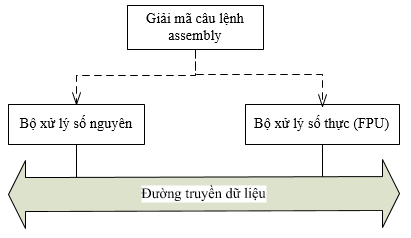
\includegraphics[scale=0.5]{FPUQuanHe.png}
				\end{center}
				\caption{Mối quan hệ giữa bộ xử lý FPU và bộ xử lý Integer}								
			\end{figure}
		\end{center}		
		
		Những câu lệnh được thực thi trong môi trường của FPU hình () bao gồm 8 thanh ghi dữ liệu (gọi là thanh ghi dữ liệu FPU) và sau đây là những thanh ghi với mục đích khác:
		\begin{itemize}
			\renewcommand{\labelitemi}{\textbullet}	
			\item	Thanh ghi trạng thái (the status register).
			\item	Thanh ghi điều khiển (the control register).
			\item	Thanh ghi thẻ (the tag word register).
			\item	Thanh ghi con trỏ lệnh (instruction poitnter register).
			\item	Thanh ghi toán hạng (last operand register).
			\item	Thanh ghi Opcode (Opcode register).
		\end{itemize}
		
	Những thanh ghi này được miêu tả trong phần tiếp theo.

		\subsubsection*{Thanh ghi dữ liệu FPU}
	Các thanh ghi dữ liệu FPU (hình 7 ) bao gồm 8 thanh ghi 80-bit. Giá trị được lưu trữ trong các thanh ghi theo định dạng mở rộng. Khi các số thực, số nguyên hoặc giá trị BCD được nén được nạp vào từ bộ nhớ vào trong thanh ghi dữ liệu FPU, các giá trị sẽ tự động chuyển về định dạng mở rộng. Khi tính toán, kết quả được chuyển lại vào bộ nhớ từ bất kỳ thanh ghi FPU, kết quả có thể đã được định dạng mở rộng hoặc được chuyển về định dạng FPU khác (số thực, số nguyên, giá trị BCD được nén).\\

	Những tập lệnh của FPU sẽ xử lý 8 thnh ghi dữ liệu nhưu là một ngăn xếp (stack) các thanh ghi (hình 7 ) tất cả địa chỉ ác thanh ghi dữ liệu là tương đối so với thanh ghi đỉnh của ngăn xếp. Số lượng thanh ghi ở đỉnh ngăn xếp hiện tại được lưu trữ trong trường TOP (stack TOP) trong thanh ghi trạng thái của FPU. Khi có 1 thao tác nạp thì TOP giảm đi 1 và nạp 1 giá trị vào thanh ghi ở đỉnh mới của ngăn xếp, và thao tác lưu trữ sẽ lưu trữ giá trị thanh ghi từ thanh ghi TOP hiện tại vào bộ nhớ.

		\subsubsection{Loại dữ liệu dấu chấm động và định dạng}
		\subsubsection{Câu lệnh FPU}	

\section{Windows API}

	\subsection{Một vài bộ thư viện cần hỗ trợ}

Ở những bước xây dựng đầu của đề tài, cần ưu tiên tiến hành cho những bộ thư viện phổ biến và được dùng rộng rãi trước tiên. Bảng 2 sau đây sẽ mô tả thông tin những bộ thư viện đã được hỗ trợ bởi BE-PUM:


\begin{longtable}{ | m{3cm} | m{11cm} | }
	\hline
Tên & Chức năng\\
	\hline
	\hline
Dịch vụ nền & Cho phép truy cập vào các nguồn tài nguyên cơ bản có sẵn trong hệ thống của Windows. Bao gồm những thứ như hệ thống tập tin, thiết bị, tiến trình (process), luồng (thread), xử lý lỗi (error handing).
Các chức năng này nằm trong tập tin kernel32.dll trên hệ điều hành Windows 32-bit.\\
	\hline
Dịch vụ nâng cao & Cho phép truy cập vào các chức năng bổ sung. Bao gồm những thứ như Windows registry, tắt/khởi động lại hệ thống (hoặc bãi bỏ - abort), bắt đầu/dừng/tạo ra một dịch vụ, quản lý tài khoản người dùng.
Các chức năng này nằm trong tập tin advapi32.dll trên hệ điều hành Windows 32-bit.\\
	\hline
Giao diện người dùng & Cung cấp các chức năng để tạo và quản lý cửa sổ màn hình và hầu hết những điều khiển cơ bản, chẳng hạn như nút và thanh cuộn, nhận chuột và bàn phím, cũng như các chức năng khác liên quan đến phần giao diện đồ họa người dùng của Windows.\\
	\hline
Các chức năng này nằm trong tập tin user32.dll trên hệ điều hành Windows 32-bit.
Windows shell & Cho phép các ứng dụng truy cập các chức năng được cung cấp bởi các shell của hệ điều hành, cũng như thay đổi nó.
Windows shell ở đây được hiểu là những thành phần cấu tạo nên giao diện đồ họa người dùng của hệ điều hành Windows (bao gồm những thứ như: màn hình desktop, thanh làm việc taskbar và các thành phần con trên nó,…).
Các chức năng này nằm trong tập tin shell32.dll trên hệ điều hành Windows 32-bit.\\
	\hline

\caption[Những bộ thư viện được hỗ trợ bởi BE-PUM]{Những bộ thư viện được hỗ trợ bởi BE-PUM}
\label{table:tblwapilib}
\end{longtable}


	\subsection{Trình tự các bước để ứng dụng JNA vào BE-PUM}

Để  tiến hành áp dụng những khả năng mang lại từ JNA và hệ thống BE-PUM, ta cần trải qua những bước sau đây:
\begin{enumerate}
	\item Ánh xạ tương ứng tên thư viện sẽ được gọi
	\item Ánh xạ tên hàm của API và những kiểu dữ liệu sẽ được dùng (bao gồm kiểu dữ liệu trả về và kiểu dữ liệu của các thông số đầu vào) từ ngôn ngữ lập trình C sang Java
	\item Tiến hành lấy giá trị bộ nhớ của các thông số đầu vào có trong BE-PUM
	\item Truyền các giá trị đó vào những kiểu tương ứng đã được ánh xạ trong Java, gọi API và lấy kết quả trả về.
	\item Lưu giá trị nhận được đó về lại bộ nhớ của BE-PUM
\end{enumerate}


	\subsection{Những kiểu dữ liệu và ánh xạ của chúng vào JNA}

Việc ánh xạ kiểu dữ liệu từ ngôn ngữ lập trình C sang Java được hỗ trợ sẵn bởi JNA cho một số kiểu cơ bản thường dùng như sau:\\

\begin{longtable}{ | m{3cm} | m{5cm} | m{5cm} | }
	\hline
STT & Kiểu dữ liệu trong C & Kiểu dữ liệu trong Java\\
	\hline
	\hline
1 & char & byte\\
	\hline
2 & wchar\_t & char\\
	\hline
3 & short & short\\
	\hline
4 & int & int\\
	\hline
5 & int & boolean\\
	\hline
6 & enum & int (thông thường)\\
	\hline
7  & long long, \_\_int64 & long\\
	\hline
8 & float & float\\
	\hline
9 & double & double\\
	\hline
10 & Con trỏ (VD: void*) & \specialcell{Buffer \\ Pointer}\\
	\hline
11 & \specialcell{Con trỏ (VD: void*, char*) \\ Mảng} & <P>[] (mảng của những kiểu nguyên thủy)\\
	\hline
12 & long & NativeLong\\
	\hline
13 & const char* & String\\
	\hline
14 & const wchar\_t* & WString\\
	\hline
15 & char** & String[]\\
	\hline
16 & wchar\_t** & WString[]\\
	\hline
17 & void** & Pointer[]\\
	\hline
18 & \specialcell{struct* \\ struct} & Structure\\
	\hline
19 & union & Union\\
	\hline
20 & struct[] & Structure[]\\
	\hline
21 & void (*FP)() & Callback\\
	\hline
22 & pointer (<T> *) & PointerType\\
	\hline

\caption[Một số ánh xạ kiểu dữ liệu cơ bản]{Một số ánh xạ kiểu dữ liệu cơ bản}
\label{table:tblwapi_type_mapping}
\end{longtable}
%\end{center}

Căn bản việc ánh xạ kiểu dữ liệu trong JNA được đáp ứng bằng việc kích thước dữ liệu được sử dụng giữa hai ngôn ngữ C và Java có kích thước bằng nhau. JNA hỗ trợ cho việc nạp một mảng các kí tự trong C bằng cách cho vào một đối tượng kiểu String.\\
 
Điểm hỗ trợ mạnh trong JNA đó là sử dụng và truy cập con trỏ của C thông qua đối tượng kiểu Pointer, dù rằng đang làm việc trong ngôn ngữ Java. Và nếu muốn lấy giá trị của một vùng nhớ thay vì chỉ một giá trị ô nhớ như Pointer, ta có thể sử dụng đối tượng kiểu Buffer để JNA đưa giá trị vùng nhớ đó vào trong đối tượng.


	\subsection{Dữ liệu kiểu cấu trúc (structure)} \label{sec:structure}

Một trong những lợi thế to lớn nhất mà JNA mang lại đó là nạp dữ liệu kiểu cấu trúc (structure) vào trong C mà ngôn ngữ Java không có. Điều này được hỗ trợ qua việc tạo ra một lớp mới, kế thừa từ lớp Structure của JNA.\\

Để tạo ra chính xác kiểu cấu trúc để nạp vào JNA, ta cũng phải tìm hiểu và nắm rõ các quy tắc xây dựng và làm việc với kiểu cấu trúc trong ngôn ngữ lập trình C.

		\begin{center}
			\begin{figure}[h]
				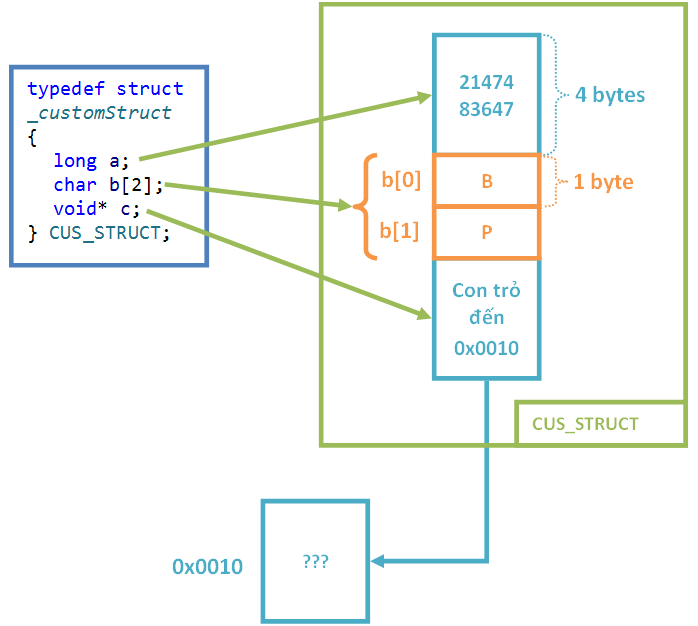
\includegraphics[scale=0.8]{StructureMemoryOrganization.png}
				\caption{Cách sắp xếp và lưu trữ bộ nhớ của structure}				
			\end{figure}
		\end{center}

Một struct trong ngôn ngữ lập trình C là một khai báo dữ liệu kiểu phức hợp, trong đó nó định nghĩa một danh sách các biến được đặt bên trong một khối bộ nhớ. Nó cho phép các biến khác nhau được truy xuất thông qua một con trỏ duy nhất (con trỏ của structure). Một structure có khả năng chứa nhiều kiểu dữ liệu khác nhau từ kiểu dữ liệu nguyên thủy đến kiểu dữ liệu phức tạp khác (enum, structure).\\

Định nghĩa struct khá giống với định nghĩa lớp trong Java, nhưng struct không hề có khả năng khai báo phương thức, cũng như các từ khóa public, private,… như Java. Thêm vào đó, cơ chế cấp phát bộ nhớ của struct chỉ đơn thuần là sự sắp xếp liên tục của các vùng nhớ chứa giá trị của các biến đã được khai báo bên trong. Cách sắp xếp này hoàn toàn tương ứng với ngôn ngữ assembly; do đó ta cần đảm bảo việc lấy ra và gán trở lại bộ nhớ BE-PUM một cách chính xác theo trình tự như vậy.

